\documentclass[12pt, leqno]{article} %% use to set typesize
\input{common}

\usepackage{fontspec}
\usepackage{polyglossia}
\setmonofont{DejaVu Sans Mono}[Scale=MatchLowercase]
\usepackage[outputdir=pdf]{minted}

\providecommand{\tightlist}{%
  \setlength{\itemsep}{0pt}\setlength{\parskip}{0pt}}
\begin{document}



\hdr{2023-04-28}

\section{Inequality constraints}

Problems with inequality constraints can be reduced to problems with
\emph{equality} constraints if we can only figure out which constraints
are active at the solution. We use two main strategies to tackle this
task:

\begin{itemize}
\tightlist
\item
  \emph{Active set} methods guess which constraints are active, then
  solve an equality-constrained problem. If the solution satisfies the
  KKT conditions, we are done. Otherwise, we update the guess of the
  active set by looking for constraint violations or negative
  multipliers. The \emph{simplex method} for linear programs is a famous
  active set method. The difficulty with these methods is that it may
  take many iterations before we arrive on the correct active set.
\item
  \emph{Interior point} methods take advantage of the fact that barrier
  formulations do not require prior knowledge of the active constraints;
  rather, the solutions converge to an appropriate boundary point as one
  changes the boundary.
\end{itemize}

Between the two, active set methods often have an edge when it is easy
to find a good guess for the constraints. Active set methods are great
for families of related problems, because they can be ``warm started''
with an initial guess for what constraints will be active and for the
solution. Many strong modern solvers are based on sequential quadratic
programming, a Newton-like method in which the model problems are
linearly-constrained quadratic programs that are solved by an active set
iteration. In contrast to active set methods, interior point methods
spend fewer iterations sorting out which constraints are active, but
each iteration may require more work.

\section{Quadratic programs with inequality constraints}

We now consider a quadratic objective with linear inequality
constraints: \begin{align*}
  \phi(x) &= \frac{1}{2} x^T H x - x^T d \\
  c(x) &= A^T x-b \leq 0,
\end{align*} where \(H \in {\mathbb{R}}^{n \times n}\) is symmetric and
positive definite, \(A \in {\mathbb{R}}^{n \times m}\) with \(m < n\),
and \(b \in {\mathbb{R}}^m\). The KKT conditions for this problem are
\begin{align*}
  Hx - d + A\lambda &= 0 \\
  A^T x-b & \leq 0 \\
  \lambda & \geq 0 \\
  \lambda_i (A^T x-b)_i &= 0.
\end{align*}

The \emph{active set} is the set of \(i\) such that \((A^T x-b)_i = 0\).
We assume that the active columns of \(A\) are always linearly
independent (e.g.~\(0 \leq x_i\) and \(x_i \leq 1\) can co-exist, but it
is not OK to have both \(x_i \leq 1\) and \(x_i \leq 2\)).

\begin{figure}
\begin{center}
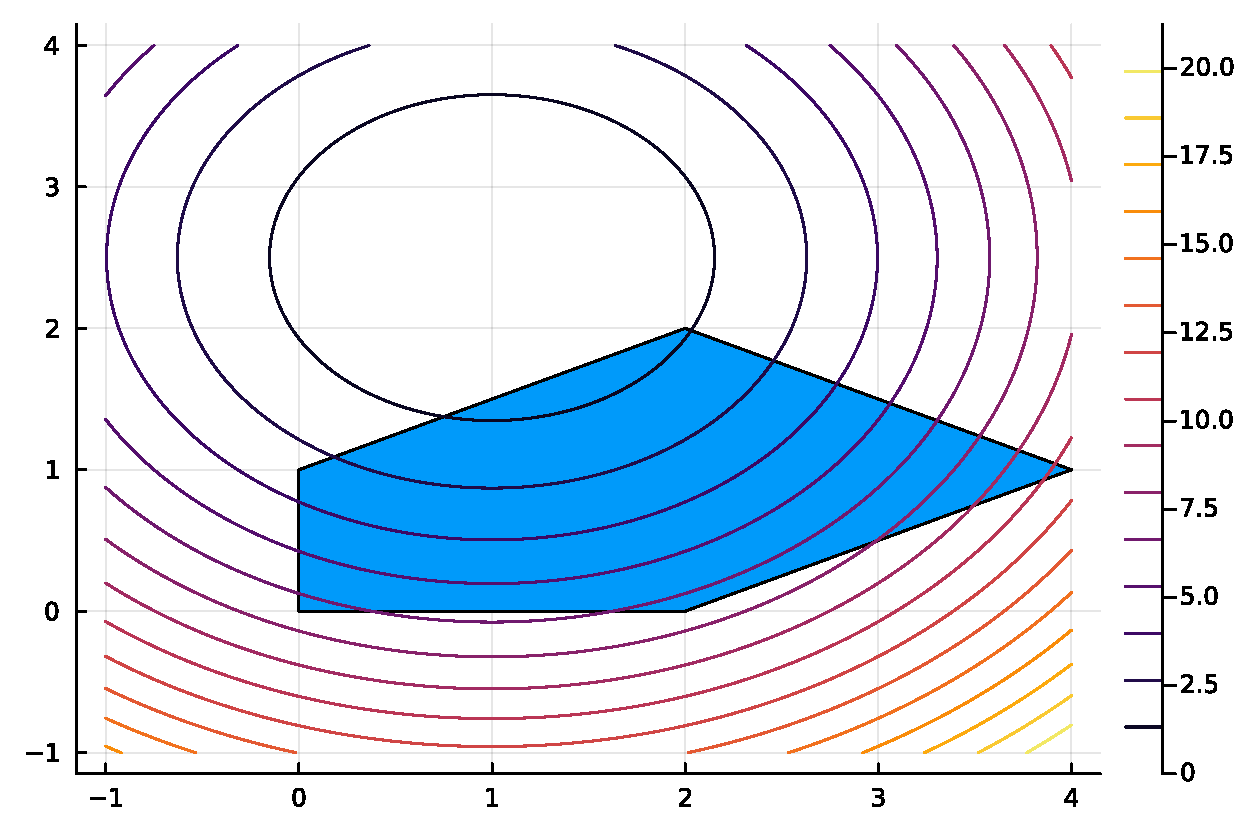
\includegraphics[width=0.8\textwidth]{fig/2023-04-28-ex16_3.pdf}
\end{center}
\caption{Example constrained quadratic problem.}
\label{fig:test-qp}
\end{figure}

Examples are always good, as are pictures.  We will borrow the
following 2D example from Nocedal and Wright (Example 16.3) -- see
Figure~\ref{fig:test-qp}.

\begin{minted}{julia}
begin
    # Objective in Nocedal and Wright: ϕ(x) = (x[1]-1.0)^2 + (x[2]-2.5)^2
    #   We will get rid of a constant term to get it to our usual form
    #   (and scale by 1/2)
    #
    H = [1.0 0.0; 0.0 1.0]
    d = [1.0; 2.5]

    # Constraints per Nocedal and Wright -- we rewrite so the inequality i
    # goes the other way
    #  x1 - 2 x2 + 2 ≥ 0
    # -x1 - 2 x2 + 6 ≥ 0
    # -x1 + 2 x2 + 2 ≥ 0
    #  x1 ≥ 0
    #  x2 ≥ 0
    #
    A = [-1.0  2.0 ;
         1.0  2.0 ;
         1.0 -2.0 ;
         -1.0  0.0 ;
         0.0 -1.0 ]'
    b = [2.0; 6.0; 2.0; 0.0; 0.0]

    # Draw a plot of the quadratic and the constraints
    function plot_ex16_3()
        q(x,y) = (x-1.0)^2 + (y-2.5)^2
        corners = [0.0 0.0 ;
                   2.0 0.0 ;
                   4.0 1.0 ;
                   2.0 2.0 ;
                   0.0 1.0 ]
        xx = range(-1.0, 4.0, length=101)
        p = plot(corners[:,1], corners[:,2], st=:shape)
        plot!(xx, xx, q, st=:contour, legend=false)
        p
    end

    plot_ex16_3()
end
\end{minted}

\section{An active set approach}

At the \(k\)th step in an active set QP solver, we update an iterate
\(x^k\) approximating the constrained minimizer \emph{and} we update a
corresponding working set \(\mathcal{W}^k\) approximating the active
set. A step of this solver looks like:

\begin{enumerate}
\def\labelenumi{\arabic{enumi}.}
\tightlist
\item
  Choose a step \(p^k\) by minimizing the quadratic form assuming the
  constraints in \(\mathcal{W}^k\) are the active constraints. This
  gives an equality-constrained subproblem.
\item
  If \(p^k\) is zero, then

  \begin{enumerate}
  \def\labelenumii{\arabic{enumii}.}
  \tightlist
  \item
    Compute the Lagrange multipliers associated with the set
    \(\mathcal{W}^k\).
  \item
    If all the multipliers are non-negative, terminate.
  \item
    Otherwise, let \(\lambda_j\) be the most negative multiplier, and
    set \(\mathcal{W}^{k+1} = \mathcal{W}^k \setminus \{ j \}\)
  \end{enumerate}
\item
  Otherwise \(p^k \neq 0\).

  \begin{enumerate}
  \def\labelenumii{\arabic{enumii}.}
  \tightlist
  \item
    Advance \(x^{k+1} = x^k + \alpha_k p^k\) where the step length
    \(\alpha_k\) is the largest allowed value (up to one) such that
    \(x^{k+1}\) is feasible.
  \item
    If \(\alpha_k < 1\), then there is (at least) one \emph{blocking
    constraint} \(j\) such that \((A^T x^{k+1}-b)_j = 0\) and
    \(j \not \in \mathcal{W}^k\). Update
    \(\mathcal{W}^{k+1} = \mathcal{W}^k \cup \{ j \}\).
  \end{enumerate}
\end{enumerate}

\begin{figure}
\begin{center}
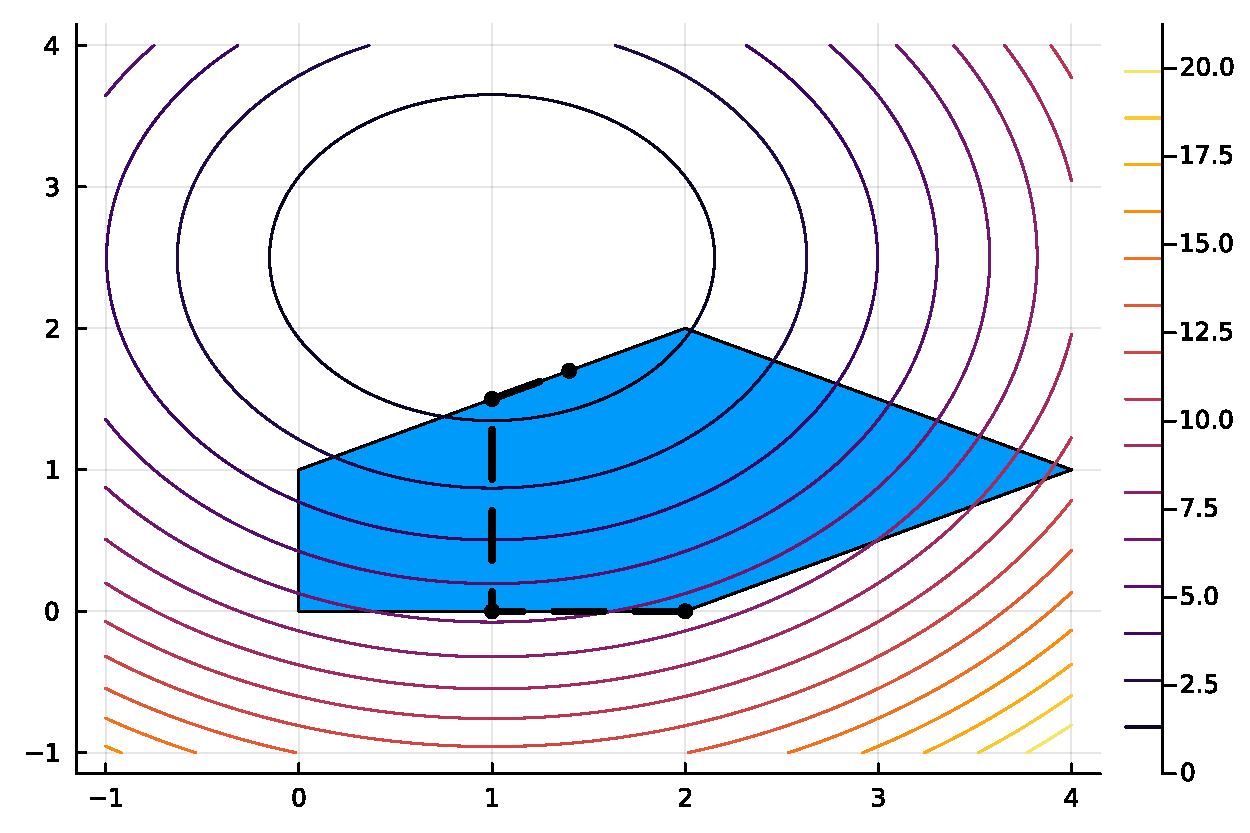
\includegraphics[width=0.8\textwidth]{fig/2023-04-28-ex16_3-as.pdf}
\end{center}
\caption{Example constrained quadratic problem and path taken by
  active set solver.}
\label{fig:test-qp-as}
\end{figure}

If we do not attempt any particular efficiency, this is mostly
straightforward to code.  Convergence for our test problem is shown
in Figure~\ref{fig:test-qp-as}

\begin{minted}{julia}
function qp_as(x0, H, d, A, b; ptol=1e-8, W0=[], nsteps=100,
               monitor=(x, W)->nothing)

    n = length(x0)
    m = length(b)
    W = zeros(Bool, m)

    x = copy(x0)
    p = zeros(n)
    λ = zeros(m)
    W[W0] .= true
    monitor(x, W)

    # Compute Cholesky factorization for range space solver
    F = cholesky(H)
    L = F.L
    Y = L\A
    c = L\d

    for k = 1:nsteps

        ## Solve the equality constrained subproblem (range space method)
        λ[:] .= 0.0
        λ[W] = ( Y[:,W]'*Y[:,W] )\( Y[:,W]'*c - b[W] )
        p[:] = L'\(c-Y[:,W]*λ[W])-x

        if norm(p) < ptol

            # Find most negative multiplier (if there is one)
            minλ = 0.0
            j = 0
            for k = 1:m
                if λ[k] < minλ
                    minλ = λ[k]
                    j = k
                end
            end

            if j == 0
                return x      # All multipliers non-negative, done!
            else
                W[j] = false  # Release jth constraint
            end

        else

            # Figure out step (and any blocking constraint)
            α = 1.0
            r = b-A'*x
            u = A'*p
            blocking_idx = 0
            for k = 1:m
                if !(k in W) && (α*u[k] > r[k])
                    α = r[k]/u[k]
                    blocking_idx = k
                end
            end

            # Take step and update list of active constraints
            x[:] += α*p
            if blocking_idx > 0
                W[blocking_idx] = true
            end
            monitor(x, W)

        end
    end
    error("Did not converge after $nsteps steps")
end
\end{minted}

A few remarks about this strategy are in order:

\begin{itemize}
\tightlist
\item
  The strategy is guaranteed not to cycle --- the working set at any
  given iterate is distinct from the working set at any other iterate.
  Assuming the steps are computed exactly (via Newton), the iteration
  converges in a finite number of steps. That said, there are an
  exponential number of working sets; and, as with the simplex method
  for linear programming, there are examples where the algorithm may
  have exponential complexity because of the cost of exploring all the
  working set. But, as with the simplex method, this is not the common
  case.
\item
  The strategy only changes the working set by adding or removing one
  constraint at a time. Hence, if \(\mathcal{A}\) is the true active
  set, the number of steps required is at least
  \(|\mathcal{W}^0| + |\mathcal{A}| - 2|\mathcal{W}^0 \cap \mathcal{A}|\).
  This is bad news if there are many possible constraints and we lack a
  good initial guess as to which ones will be active.
\item
  If we compute the steps \(p^k\) as described above, the cost per step
  (after an initial factorization of the Hessian and triangular solves
  on the constraints) would appear to be \(O(n^2+n|\mathcal{W}^k|^2)\).
  In practice, though, each linear system differs from the previous
  system only through the addition or deletion of a constraint. If we
  are clever with our numerical linear algebra, and re-use the
  factorization work already invested through updating and downdating,
  we can reduce the cost per step.
\end{itemize}

\section{Barriers: hard and soft}

Before we proceed, a word is in order about the relationship between
Lagrange multipliers and barriers or penalties. To be concrete, let us
consider the inequality-constrained problem
\[\mbox{minimize } \phi(x) \mbox{ s.t. } c(x) \leq 0,\] where
\(c : {\mathbb{R}}^n \rightarrow {\mathbb{R}}^m\) with \(m < n\), and
the inequality should be interpreted elementwise. In a barrier
formulation, we approximate the problem by problems of the form
\[\mbox{minimize } \phi(x) - \mu \sum_{j=1}^m \log(-c_j(x)),\] where the
second term shoots to infinity as \(c_j(x) \rightarrow 0\); but for any
fixed \(c_j(x) < 0\) it becomes negligible once \(\mu\) is small enough.
Differentiating this objective gives us the critical point equations
\[\nabla \phi(\hat{x}(\mu))
  -\sum_{j=1}^m \frac{\mu}{c_j(\hat{x}(\mu))} \nabla c_j(\hat{x}(\mu)) = 0.\]
By way of comparison, if we were to try to exactly optimize this
inequality constrained problem, we would want to satisfy the KKT
conditions \begin{align*}
  \nabla \phi(x) + \nabla c(x) \lambda &= 0 \\
  c(x) & \leq 0 \\
  \lambda & \geq 0 \\
  \lambda_j(x) c_j(x) &= 0.
\end{align*} Comparing the two, we see that the quantities
\(\hat{\lambda}_j(\mu) \equiv -\mu/c_j(x_*(\mu))\) should approximate
the Lagrange multipliers: they play the same role in the equation
involving the gradient of \(\phi\), they are always positive for
\(\mu > 0\), and \(\hat{\lambda}_j(x_*(\mu)) \rightarrow 0\) provided
\(c_j(x_*(\mu)) \not \rightarrow 0\).

I like to think of barriers and penalties in physical terms as being
like slightly flexible walls. In real life, when you push on a wall,
however stiff, there is a little bit of give. What we see as an opposing
force generated by a rigid wall is really associated with that little
bit of elastic give. But a good idealization is that of a perfectly
rigid wall, which does not give at all. Instead, it responds to conctact
with exactly the amount of force normal to the wall surface that is
required to counter any force pushing into the wall. That
equal-and-opposite force is exactly what is captured by Lagrange
multipliers, where the very stiff elastic response is captured by the
barrier or penalty formulation, with the parameter \(\mu\) representing
the compliance of the barrier (inverse stiffness).

The weakness of a penalty or barrier approach is two-fold: if \(\mu\) is
far from zero, we have a thick and spongy barrier (a poor approximation
to the infinitely rigid case); whereas if \(\mu\) is close to zero, we
have a nearly-rigid barrier, but the Hessian of the augmented barrier
function becomes very ill-conditioned, scaling like \(\mu^{-1}\). In
contrast, with a Lagrange multiplier formulation, we have a perfect
barrier and no problems with ill-conditioning, but at the cost of having
to explicitly determine whether the optimum is at one or more of the
constraint surfaces, and also what ``contact forces'' are needed to
balance the negative gradient of \(\phi\) that pushes into the barrier.

Several modern algorithmic approaches, such as augmented Lagrangian and
interior point methods, get the best of both perspectives by combining a
penalty or barrier term with a Lagrange multiplier computation.

\section{An interior point strategy}

Having touched on the relation between Lagrange multipliers and
logarithmic barriers, let us now turn to an interior point method for
quadratic programming. We start by rewriting the constraints
\(A^Tx - b \leq 0\) in terms of an extra set of slack variables:
\[y = b-A^Tx \geq 0.\] With this definition, we write the KKT conditions
as \begin{align*}
  Hx - d + A\lambda & = 0 \\
  A^T x-b+y &= 0 \\
  \lambda_i y_i &= 0 \\
  y_i, \lambda_i & \geq 0.
\end{align*} Interior point methods solve this system by applying
Newton-like iterations to the three equations, while at the same time
ensuring that the inequalities are enforced strictly at every step (that
is, every step is interior to the feasible domain).

Compare this to the critical point conditions for the barrier problem
\[\mbox{minimize } \frac{1}{2} x^T H x - x^T d - \gamma \sum_{j=1}^m \log(y_j)\]
for some small value of the barrier parameter \(\gamma\), where we note
that \[\nabla_x \left( -\gamma \sum_{j=1}^n \log(y_j) \right) =
  A \hat{\lambda}, \quad \hat{\lambda}_j = \frac{\gamma}{y_j}\] and we
can rewrite this system as \begin{align*}
  Hx - d + A\hat{\lambda} &= 0 \\
  A^T x - b + y &= 0 \\
  y_i \hat{\lambda}_i - \gamma &= 0.
\end{align*} Typical interior point methods take guarded Newton steps
(or Newton-like steps) on this system of equations, which can be
regarded as a relaxation of the KKT conditions or as a critical point of
a barrier formulation. The path traced out as \(\mu\) varies is known as
the ``central path.''

\begin{figure}
\begin{center}
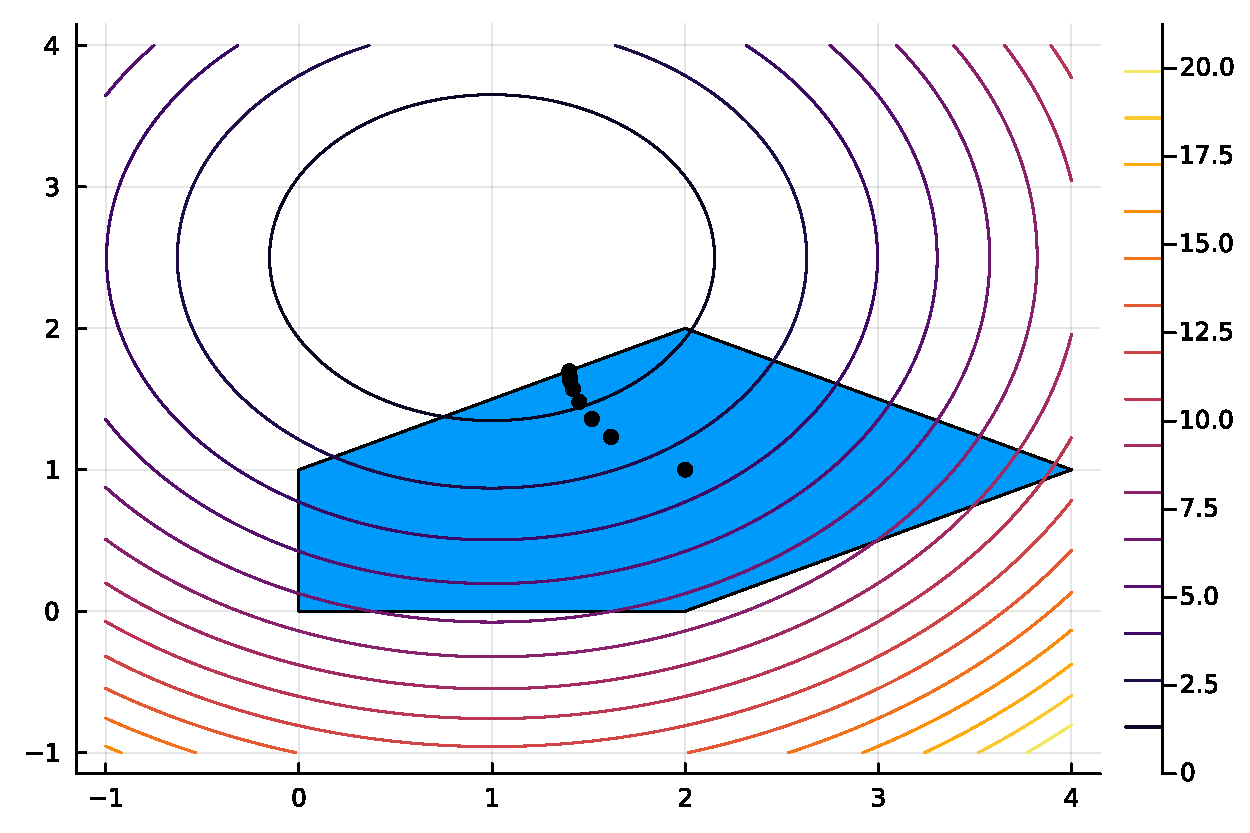
\includegraphics[width=0.8\textwidth]{fig/2023-04-28-ex16_3-ip.pdf}
\end{center}
\caption{Example constrained quadratic problem with central path.}
\label{fig:test-qp-ip}
\end{figure}

We plot the central path taken for our test problem in
Figure~\ref{fig:test-qp-ip}.

\begin{minted}{julia}
function barrier_qp(x0, H, d, A, b, γ; nsteps=20, ptol=1e-8)

    n = length(d)
    m = length(b)
    σ = 0.5

    x = copy(x0)
    y = b-A'*x
    λ = γ./y

    F(x, y, λ) = [H*x - d + A*λ;
                  A'*x - b + y;
                  y.*λ .- γ]
    J(x, y, λ) = [H          zeros(n,m)  A;
                  A'         I           zeros(m,m);
                  zeros(m,n) diagm(λ)    diagm(y)]

    α = 1.0
    p = -(J(x, y, λ) \ F(x, y, λ))
    for k = 1:nsteps
        xnew = x + α*p[1:n]
        if all(A'*xnew-b .<= 0.0)
            x = xnew
            y += α*p[n+1:n+m]
            λ += α*p[n+m+1:end]
            if α == 1.0 && norm(p) < ptol
                return x, λ
            end
            α = 1.0
            p = -(J(x, y, λ) \ F(x, y, λ))
        else
            α /= 2.0
        end
    end

    error("Did not converge in $nsteps steps")
end
\end{minted}

The parameter \(\gamma\) is adjusted dynamically during the solve, and
is usually written as \(\gamma = \sigma \mu\) where \(\sigma \in [0,1]\)
is the centering parameters and \(\mu = y^T \lambda / m\) is the
\emph{complimentarity measure}, which should go to zero as we approach a
problem solution. Getting all the details right is somewhat complicated,
though, and we recommend using a package written by someone with some
expertise.

Interior point methods avoid the problem of having to do a combinatorial
search to figure out the correct active set. At the same time, active
set methods may be more efficient for problems where we have a good
initial guess at the active set. Neither approach is universally
preferable. Indeed, it is possible to take a hybrid approach where an
interior point method (or something similar) is used to estimate which
constraints are actually active, and then an active set method serves to
``clean up'' the solution.


\end{document}
